\chapter{Testing}
\label{cha:400}
In the following sections there are all the cases considered, with a brief definition of the tasks, and are present the configuration settings used for each specific environment. Finally the results of the tests were reported for each case and there are some consideration deduced from them, with the last section containing the interpretability study, which is a key aspect in IAI.

What I expected is that PPO would be able to optimize a lot of the individuals given to it, even if they wouldn't be able to solve completely the task, because the orthogonal DTs with constant leaves used are often too simple to solve the more complex environments. Despite this premise, I expected that sometimes, for the simplest environment (i.e. CartPole-v1) PPO would produce a DT with a maximum fitness, solving the task.

For this work, it were considered three environments, two have a sparse reward and the other one not, to see how PPO behaves in these two different situations.

\textit{Note:} all the environments considered has a discrete action space.


\section{CartPole-v1}
\label{sec:410}
\subsection{Definition}
\label{subsec:411}
A pole is attached by an un-actuated joint to a cart, which moves along a frictionless track. The pendulum is placed upright on the cart and the goal is to balance the pole by applying forces in the left and right direction on the cart \cite{gym} \cite{cartpole}.\\[0.3in]
The \textit{\textbf{state}} of the environment has dimension equals to 4 and is composed of:
\begin{itemize}
    \item Cart position: \textit{x} \(\in\) [-4.8, 4.8] m
    \item Cart velocity: \textit{v} \(\in\) ]-\(\infty\), \(\infty\)[ m/s
    \item Pole angle: \textit{\(\theta\)} \(\in\) [-0.418, 0.418] rad
    \item Pole angular velocity: \textit{\(\omega\)} \(\in\) ]-\(\infty\), \(\infty\)[ rad/s
\end{itemize}
The \textit{\textbf{actions}} that the agent can perform are:
\begin{itemize}
    \item Move left (applying a 10N force to the cart)
    \item Move right (applying a 10N force to the cart)
\end{itemize}
The agent receives a \textit{\textbf{reward}} of +1 for every step taken.\\[0.1in]
The \textit{\textbf{termination criterion}} is one of the following:
\begin{itemize}
    \item Pole angle \textit{$\theta$} is greater than $\pm$ 0.2095 rad
    \item Cart position \textit{x} is greater than $\pm$ 2.4 (center of the cart reaches the edge of the display)
    \item Episode length is greater than 500
\end{itemize}
The task is considered \textit{\textbf{solved}} if the agent obtains a mean reward \textit{R} \(\geq\) 475 on 100 runs.


\subsection{Settings}
\label{subsec:412}
The grammar used is shown in the Table \ref{table:1}. The settings used for GE is shown in the Table \ref{table:2}. The parameters are taken from \cite{custode} and was made a modification for some of them by a manual tuning.
\newpage


\captionsetup{margin=2cm}
\begin{table}[h!]
\begin{center}
\begin{tabular}{ |c|c| }
\hline
\textbf{Rule} & \textbf{Production} \\
\hline
dt & \textit{$< if >$}\\
if & \textit{$if < condition > then < action > else < action >$}\\
condition & \textit{lt$(input\_feature,<constant>)$}\\
action & \textit{leaf $| < if >$}\\
constant & $[-4.8, 4.8]$ with step 0.005\\
\hline
\end{tabular}
\caption{Grammar used to evolve orthogonal decision trees in the CartPole-v1 environment. The symbol "$|$" indicates that there is the possibility to choose between different symbols. Input\_feature stands for one of the possible inputs taken from the state space.}
\label{table:1}
\end{center}
\end{table}


\begin{table}[h!]
\begin{center}
\begin{tabular}{ |c|c| } 
\hline
\textbf{Parameter} & \textbf{Value} \\
\hline
Population size & 200\\
Generations & 200\\
Genotype length & 100\\
Crossover probability & 0\\
Mutation probability & 1\\
Mutation type & Uniform, with gene probability = 0.1\\
PPO & every 40 generations\\
\hline
\end{tabular}
\caption{Parameters used for the Grammatical Evolution with orthogonal decision trees in the CartPole-v1 environment.}
\label{table:2}
\end{center}
\end{table}


\subsection{Results}
\label{subsec:413}
The results are shown in the Table \ref{table:scoreCP}. For the considerations made in chapter \ref{cha:300}, they take into account not only the fitness of individuals optimized with GE, but also the ones from PPO.

The task was solved by the agent 9 times on 10 runs ($90\%$ of the cases), with only a low fitness on Run2. In particular PPO was applied every 40 generations, so 4 times per run for a total of 40 PPO runs during all the training processes. Of these 40, in 29 runs PPO brought an improvement of the fitness of the individuals and in 4 of these 29 runs it has generated a maximum score in the generations in which it was applied.

To better see the optimization that PPO has done to individuals, in Figure \ref{fig:ComparisonSingleCP} are shown in particular 3 runs of the 10 runs made in which PPO greatly affects the convergence towards the solved threshold. In this figure is possible to notice, looking for example the fitness for the best individual of Run4, that it reached the state-of-the-art reward during the 40th generation, thanks to PPO; comparing it with the same test, without using PPO, it reached the state of the art only during the 128th generation, so 88 generations later. In this case, PPO was able to save the $68.75\%$ of generations, which is a huge improvement. Similar cases are Run1 and Run3.

In Figure \ref{fig:BestTreeCP} is shown the best DT obtained from PPO for the Run4, during the 40th generation (the case discussed before): before applying PPO, it had a fitness of 9.4 and after the algorithm has been applied, it obtains a score of 499.8, averaged on 100 unseen episodes in the environment, solving the task. This demonstrates that sometimes a particular genotype contains the potential to gain an high score, having good \textit{input\_features} in the decision nodes and need only small changes on \textit{split\_values} or in constant leaves: in fact PPO, in this case, changed some actions contained in the leaves (from \textit{move\_left} to \textit{move\_right} or vice versa) and this led to an enormous improvement in terms of fitness because it upended completely the behaviour of the individual.

Finally in the Figure \ref{fig:CartPoleMean} is shown the training mean best fitness for each generation averaged across all the 10 runs. The orthogonal decision trees are able to converge to the fitness threshold which indicates that the task is solved.

Differently from results in \cite{custode}, here the algorithm takes more generations to converge and also in a case it wasn't able to create in time a policy to solve the task: mainly this is due to the fact that I used constant leaves for this work, while in that paper were used \textit{QLearningLeaves}, so the leaves were able to learn the best action using the Q Learning algorithm.

Concluding, with the promising results obtained via PPO shown above, I can say that if it had been possible to put back into the population all the optimized individuals from PPO, using them to do crossover or mutation, the whole evolutionary algorithm would have benefited from it, reducing the number of generations needed to converge towards this threshold.

To see the complete version of the DT in Figure \ref{fig:BestTreeCP} and how it was pruned, look at the supplementary material.
\vspace{0.3in}

\begin{table}[h!]
\begin{center}
\begin{tabular}{ |c|c|c|c|c| } 
\hline
\textbf{Run} & \textbf{Seed} & \textbf{Training Best Fitness} & \textbf{Testing Best Fitness} & $\mathcal{M}$\\
\hline
R1 & 0 & \textbf{500.00} & \textbf{500.00} & 53.4\\
R2 & 1 & 234.8 & 199.71 & 35.6\\
R3 & 2 & \textbf{500.00} & \textbf{487.40} & 53.4\\
R4 & 3 & \textbf{500.00} & \textbf{499.28} & 53.4\\
R5 & 4 & \textbf{500.00} & \textbf{488.20} & 35.6\\
R6 & 5 & \textbf{500.00} & \textbf{498.05} & 53.4\\
R7 & 6 & \textbf{500.00} & \textbf{486.26} & 53.4\\
R8 & 7 & \textbf{500.00} & \textbf{500.00} & 35.6\\
R9 & 8 & \textbf{500.00} & \textbf{493.96} & 53.4\\
R10 & 9 & \textbf{500.00} & \textbf{498.8} & 53.4\\
\hline
\end{tabular}
\caption{Reward obtained by the best policy with orthogonal decision trees on CartPole-v1 environment (bold denotes the solved ones)}
\label{table:scoreCP}
\end{center}
\end{table}

\begin{figure}[h!]
    \centering
    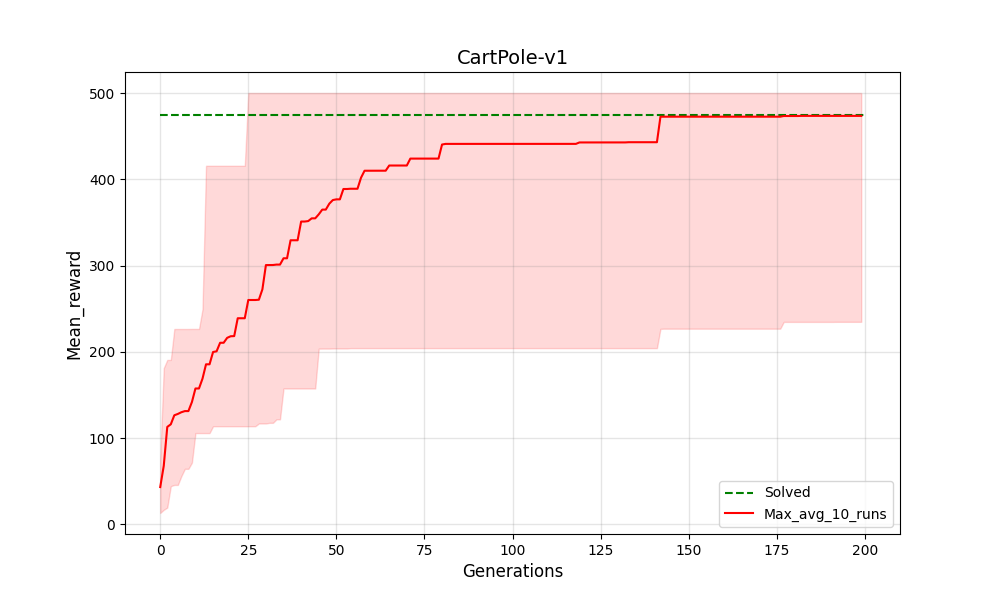
\includegraphics[width=1\linewidth]{images/CartPole/CartPole10run.png}
    \caption{Total training mean reward with orthogonal decision trees in the CartPole-v1 environment, using both GE and PPO}
    \label{fig:CartPoleMean}
\end{figure}

\newpage

\begin{figure}[h!]
    \centering
    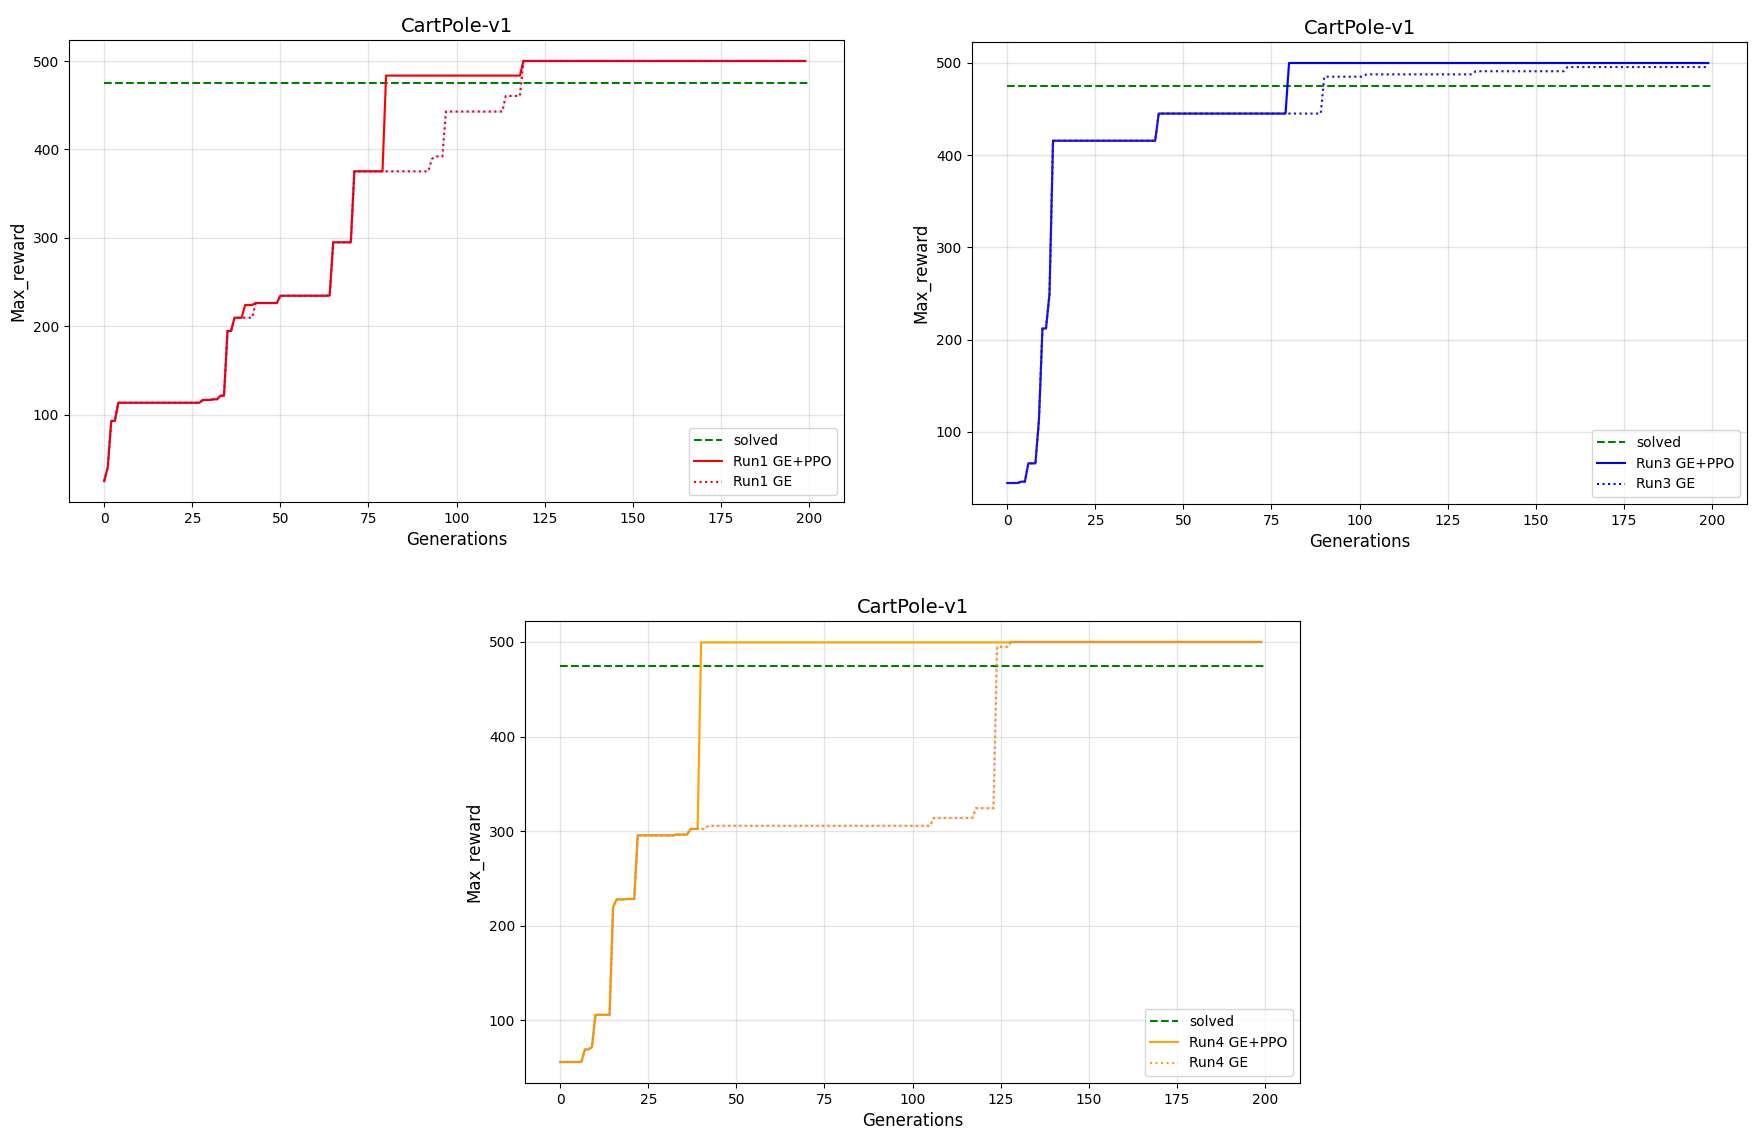
\includegraphics[width=1\linewidth]{images/CartPole/mixedRunSingle.png}
    \caption{Comparison between fitnesses for Run1, Run3 and Run4. The solid line represents the results using both GE and PPO, instead the dotted line represents the results considering only GE}
    \label{fig:ComparisonSingleCP}
\end{figure}

\begin{figure}[h!]
    \centering
    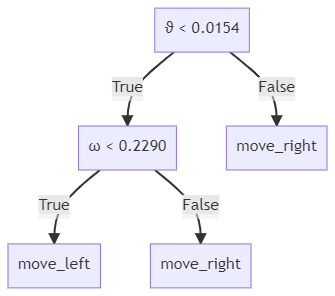
\includegraphics[width=0.4\linewidth]{images/CartPole/bestPPOprunedCP.png}
    \caption{The best tree optimized by PPO in CartPole-v1 environment, pruned by eliminating unnecessary branches}
    \label{fig:BestTreeCP}
\end{figure}

\newpage



\section{Acrobot-v1}
\label{sec:420}
\subsection{Definition}
\label{subsec:421}
The system consists of two links connected linearly to form a chain, with one end of the chain fixed. The joint between the two links is actuated. The goal is to apply torques on the actuated joint to swing the free end of the linear chain above a given height while starting from the initial state of hanging downwards \cite{gym} \cite{acrobot} \cite{sutton}.\\[0.3in]
The \textit{\textbf{state}} of the environment has dimension equals to 6 and is composed of:
\begin{itemize}
    \item Cosine of \(\theta_1\): \textit{cos(\(\theta_1\))} \(\in\) [-1, 1]
    \item Sine of \(\theta_1\): \textit{\(sin(\theta_1\))} \(\in\) [-1, 1]
    \item Cosine of \(\theta_2\): \textit{cos(\(\theta_2\))} \(\in\) [-1, 1]
    \item Sine of \(\theta_2\): \textit{sin(\(\theta_2\))} \(\in\) [-1, 1]
    \item Angular velocity of \(\theta_1\): \textit{\(\omega_1\)} \(\in\) [-4\(\cdot\pi\), 4\(\cdot\pi\)] rad/s
    \item Angular velocity of \(\theta_2\): \textit{\(\omega_2\)} \(\in\) [-9\(\cdot\pi\), 9\(\cdot\pi\)] rad/s
\end{itemize}
The \textit{\textbf{actions}} that the agent can perform are:
\begin{itemize}
    \item Apply -1 torque to the actuated joint
    \item Apply 0 torque to the actuated joint
    \item Apply 1 torque to the actuated joint
\end{itemize}
The agent receives a \textit{\textbf{reward}} of -1 for each timestep. When it reaches the target height, it receives a reward equals to 0.\\[0.1in]
The \textit{\textbf{termination criterion}} is one of the following:
\begin{itemize}
    \item The free end reaches the target height, which is constructed as: \(-\cos(\theta_1) - \cos(\theta_2 + \theta_1) > 1.0\)
    \item Episode length is greater than 500
\end{itemize}
The task is considered \textit{\textbf{solved}} if the agent obtains a mean reward \textit{R} \(\geq\) -100 on 100 runs.


\subsection{Settings}
\label{subsec:422}
The grammar used is shown in the Table \ref{table:5}. The settings used for GE is shown in the Table \ref{table:6}. The parameters were found by a manual tuning.


\captionsetup{margin=2cm}
\begin{table}[h!]
\begin{center}
\begin{tabular}{ |c|c| }
\hline
\textbf{Rule} & \textbf{Production} \\
\hline
dt & \textit{$< if >$}\\
if & \textit{$if < condition > then < action > else < action >$}\\
condition & \textit{lt$(input\_feature,<constant>)$}\\
action & \textit{leaf $| < if >$}\\
constant & $[-28.27, 28.27]$ with step 0.001\\
\hline
\end{tabular}
\caption{Grammar used to evolve orthogonal decision trees in the Acrobot-v1 environment. The symbol "$|$" indicates that there is the possibility to choose between different symbols. Input\_feature stands for one of the possible inputs taken from the state space.}
\label{table:5}
\end{center}
\end{table}


\begin{table}[h!]
\begin{center}
\begin{tabular}{ |c|c| } 
\hline
\textbf{Parameter} & \textbf{Value} \\
\hline
Population size & 200\\
Generations & 50\\
Genotype length & 100\\
Crossover probability & 0\\
Mutation probability & 1\\
Mutation type & Uniform, with gene probability = 0.1\\
PPO & every 15 generations\\
\hline
\end{tabular}
\caption{Parameters used for the Grammatical Evolution with orthogonal decision trees in the Acrobot-v1 environment.}
\label{table:6}
\end{center}
\end{table}


\subsection{Results}
\label{subsec:423}
The results are shown in the Table \ref{table:scoreAB}. The task was solved by the agent in $100\%$ of the cases, during 10 runs. This result doesn't surprise me, being Acrobot-v1 an environment little more complex than CartPole-v1 environment (because it has an higher input and action dimension), but still an easy one.

PPO was applied every 15 generations, so 3 times per run for a total of 30 PPO runs during all the training processes. During this 30 runs, in the majority of the cases PPO was not able to improve the individuals (lowering the fitness of the individual or maintaining the previous one), with only a few weak optimizations, resulting in a non efficient process.

In addition, PPO has never obtained an individual that has the best fitness for the generation in progress, so it didn't accelerate really the process to converge the maximum fitness to the optimal one. This last statement is obvious also because I applied PPO starting from the 15th generation onward and, looking the plot of the fitnesses in Figure \ref{fig:AcrobotMean}, it's possible to notice that the average max during all the runs has passed the solved threshold very quickly, around the 8th-9th generation.

Despite this, PPO could also have found a new maximum for the evolutionary process (as it happened for CartPole-v1), but unfortunately was not this the case.

In total, PPO never improved an individual by getting it to solve the task; I reported the best one optimized via PPO in Figure \ref{fig:BestTreeAB}, in a pruned version, even if its average reward during the testing phase in the environment is lower than the -100.0 solved threshold (it obtains a reward equals to -113.89, averaged on 100 unseen episodes). Looking at each single score in the environment, I discovered that in 36 of this 100 testing runs, the model was able to solve the task, also obtaining sometimes the maximum reward of -81.0; on the other hand, it also obtained sometimes -245.0, which greatly lowers the total mean; this denotes that the policy is not steady enough, leading to solve the task only occasionally.

The original policy was deeper and more complex and is visible in the Figure \ref{fig:TreeFullAB} in the appendix, but many branches were impossible to take, so they have been pruned off, obtaining a tree with depth equals to 3 (for the full simplification process, see the dedicated appendix section).

Talking about the motivation for which the results from PPO are so negative, this is due to the fact that the Acrobot-v1 environment, as MountainCar-v0, has a sparse reward: this means that the reward is obtained from the environment only if it can reach the termination criterion (for this environment is that the free end reaches a target height), differently from CartPole-v1. Being PPO an on-policy algorithm, it means that it collects data from a certain amount of episodes and after it performs a policy gradient update. Reaching the target height with random actions (obtained from a random policy) or a non perfectly optimized policy (the ones that are sent to PPO) is a really rare event and when it happens, it's unlikely that a single positive reward affects the process so much. This leads PPO to get stuck for the majority of the times during the entire optimization process and explains the bad results overall.

This statement was confirmed in \cite{ppo_acrobot}, where the author was not able to solve the Acrobot-v1 task with PPO, and the reason was corroborated in \cite{ppo_mountaincar}.

For this reason it was also added a constraint, in addition to those present in the Section \ref{sec:330}, to the individuals that could be optimized via PPO, to improve the process; the additional constraint is that the random individual to be chosen cannot have a fitness equals to -500.0 (the lowest for the Acrobot-v1 environment). In this way I helped a bit the optimization process, being sometimes useful to improve, even a bit, some individuals.

In conclusion, it was not worth applying PPO in this environment due to the sparse reward and the algorithm didn't help the fitness to reach the solved threshold, although the task is one of the easiest in the \textit{Classic Control} library.
\vspace{0.3in}

\begin{table}[h!]
\begin{center}
\begin{tabular}{ |c|c|c|c|c| } 
\hline
\textbf{Run} & \textbf{Seed} & \textbf{Training Best Fitness} & \textbf{Testing Best Fitness} & $\mathcal{M}$\\
\hline
R1 & 0 & \textbf{-81.0} & \textbf{-83.43} & 35.6\\
R2 & 1 & \textbf{-80.0} & \textbf{-88.71} & 35.6\\
R3 & 2 & \textbf{-81.2} & \textbf{-88.07} & 35.6\\
R4 & 3 & \textbf{-75.4} & \textbf{-84.85} & 71.2\\
R5 & 4 & \textbf{-76.4} & \textbf{-82.32} & 35.6\\
R6 & 5 & \textbf{-83.6} & \textbf{-84.23} & 17.8\\
R7 & 6 & \textbf{-74.2} & \textbf{-83.94} & 35.6\\
R8 & 7 & \textbf{-70.4} & \textbf{-87.91} & 35.6\\
R9 & 8 & \textbf{-83.0} & \textbf{-83.87} & 35.6\\
R10 & 9 & \textbf{-87.6} & \textbf{-85.03} & 53.4\\
\hline
\end{tabular}
\caption{Reward obtained by the best policy with orthogonal decision trees on Acrobot-v1 environment (bold denotes the solved ones)}
\label{table:scoreAB}
\end{center}
\end{table}


\begin{figure}[h!]
    \centering
    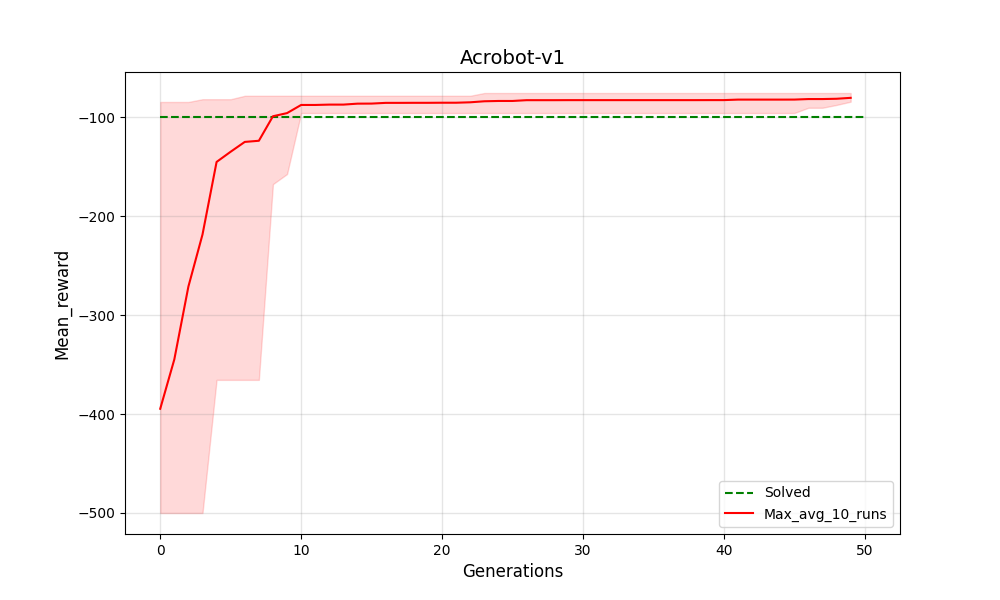
\includegraphics[width=1\linewidth]{images/Acrobot/Acrobot10run.png}
    \caption{Total training mean reward with orthogonal decision trees in the Acrobot-v1 environment, using both GE and PPO}
    \label{fig:AcrobotMean}
\end{figure}

\begin{figure}[h!]
    \centering
    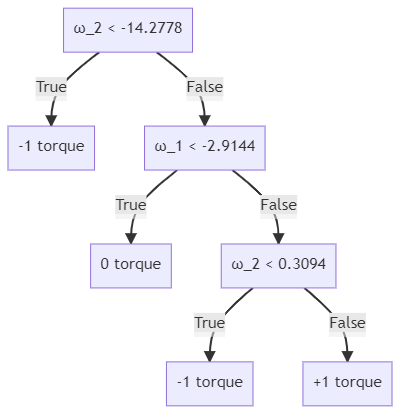
\includegraphics[width=0.4\linewidth]{images/Acrobot/bestPPOprunedAB.png}
    \caption{The best tree optimized by PPO in Acrobot-v1 environment, pruned by eliminating unnecessary branches}
    \label{fig:BestTreeAB}
\end{figure}

\newpage

\section{MountainCar-v0}
\label{sec:430}
\subsection{Definition}
\label{subsec:431}
The Mountain Car MDP is a deterministic MDP that consists of a car placed stochastically at the bottom of a sinusoidal valley, with the only possible actions being the accelerations that can be applied to the car in either direction. The goal of the MDP is to strategically accelerate the car to reach the goal state on top of the right hill \cite{gym} \cite{mountaincar}.\\[0.3in]
The \textit{\textbf{state}} of the environment has dimension equals to 2 and is composed of:
\begin{itemize}
    \item Position of the car along the x-axis: \textit{x} \(\in\) [-1.2, 0.6] m
    \item Velocity of the car: \textit{v} \(\in\) [-0.07, 0.07] m/s
\end{itemize}
The \textit{\textbf{actions}} that the agent can perform are:
\begin{itemize}
    \item Accelerate to the left
    \item Don't accelerate
    \item Accelerate to the right
\end{itemize}
The agent is penalised receiving a \textit{\textbf{reward}} of -1 for each timestep.\\[0.1in]
The \textit{\textbf{termination criterion}} is one of the following:
\begin{itemize}
    \item Episode length is greater than 200 timesteps
    \item The position of the car is greater than or equal to 0.5 (the goal horizontal position on top of the right hill)
\end{itemize}
The task is considered \textit{\textbf{solved}} if the agent obtains a mean reward \textit{R} \(\geq\) -110 on 100 runs.


\subsection{Settings}
\label{subsec:432}
The grammar used is shown in the Table \ref{table:3}. The settings used for GE is shown in the Table \ref{table:4}. The parameters are taken from \cite{custode} and was made a modification for some of them by a manual tuning.


\captionsetup{margin=1.7cm}
\begin{table}[h!]
\begin{center}
\begin{tabular}{ |c|c| }
\hline
\textbf{Rule} & \textbf{Production} \\
\hline
dt & \textit{$< if >$}\\
if & \textit{$if < condition > then < action > else < action >$}\\
condition & \textit{lt$(input\_feature,<constant>)$}\\
action & \textit{leaf $| < if >$}\\
constant & $[-1.2, 0.6]$ with step 0.005\\
\hline
\end{tabular}
\caption{Grammar used to evolve orthogonal decision trees in the MountainCar-v0 environment. The symbol "$|$" indicates that there is the possibility to choose between different symbols. Input\_feature stands for one of the possible inputs taken from the state space.}
\label{table:3}
\end{center}
\end{table}


\begin{table}[h!]
\begin{center}
\begin{tabular}{ |c|c| } 
\hline
\textbf{Parameter} & \textbf{Value} \\
\hline
Population size & 200\\
Generations & 1000\\
Genotype length & 1024\\
Crossover probability & 0\\
Mutation probability & 1\\
Mutation type & Uniform, with gene probability = 0.05\\
PPO & in the 50th-100th-400th-800th generation\\
\hline
\end{tabular}
\caption{Parameters used for the Grammatical Evolution with orthogonal decision trees in the MountainCar-v0 environment.}
\label{table:4}
\end{center}
\end{table}

\subsection{Results}
\label{subsec:433}
The results are shown in the Table \ref{table:scoreMC}. As for all the others environment, also here the results take in account the optimized individuals from PPO.

In this case, the task was much more difficult than the previous ones: for this reason, it was needed to increase not only the number of generations of the process, but also the maximum genotype length to be able to obtain more complex DTs. Those modifications are shown in the configuration settings for GE in the Table \ref{table:4}. A consequence of raising those parameters is obviously that the evolutionary process takes more time to be carried out; moreover, increasing the maximum genotype length slows down the "decision" process, because the trees generated from the algorithm could have very high depth and it takes more time to visit all the nodes that are needed to take the decision (remember that during PPO optimization all the nodes are visited for each decision that has to be taken).

\textit{Note:} also in this experiment I added the same constraint as the one added in Acrobot-v1 environment (that the individuals with the minimum fitness cannot be optimized by PPO) because also MountainCar has a sparse reward and for this reason PPO does not work well being an on-policy algorithm, as explained by \cite{ppo_mountaincar}. This additional condition helps a bit the optimization process, not wasting time on that type of individuals.

The task was solved in the $50\%$ of the cases, during 10 runs (in all the runs where it wasn't able to solve the task, the optimization has stalled with a policy that obtains a reward very close to the solved threshold).

In total, PPO was applied 4 times every run, for a total of 40 PPO runs (39 to be precise, because, during the 50th generation on the 6th run, no individuals of the populations met all the constraint defined in the Section \ref{sec:330}).

For this experiment, I decided not to apply PPO every \textit{"n"} generations but I choose to put the optimization process via PPO in specific points (4 in all, in line with the other tests), during the 50th, the 100th, the 400th and the 800th generation. I chose those particular generations because I wanted to optimize the population during different phases of the evolutionary process: the first two seek to speed up the convergence towards the solved threshold; the other two placed at the 400th and at the 800th generation, when the algorithm has probably already solved the task, try to improve the final result (getting the state-of-the-art) or possibly try to unlock a process that was stuck with a policy for a long time.

Talking about the optimization during the 50th and the 100th generations, it was during those generations (the 50th on the 3rd run precisely) that I gained the best tree from PPO and it is shown in the Figure \ref{fig:BestTreeMC}, in a simplified version. The DT, before the optimization, has a fitness equals to -117.3, so it does not solve the task, but after PPO was applied, then it was tested on 100 unseen episodes and obtain a mean reward of -107.89, being the best tree not only for that particular generation, but also for the whole evolutionary process. Even if the mean reward was under the threshold and so it correctly solves the task for the definition made in Section \ref{subsec:431}, looking at each single reward, it happens that sometimes the policy was not been able to solve the task in time (it went a bit over the threshold). Probably this is due to the fact that the DT obtained is not complex enough to solve the task with any seed, because it lacks some condition that covers each different scenario: in fact, comparing the tree with the best obtained in \cite{custode}, shown in Figure \ref{fig:BestTreeLLCMC}, it's possible to notice that the left subtree is approximately the same (same \textit{input\_features}, same actions in leaves and very similar \textit{split\_values}), but on the right subtree, there are two additional condition nodes, which give to the policy the complexity needed to solve the task in each situation.

Unfortunately, all the other times that PPO was applied, it did not lead to a significant improvement, but only achieved small enhancements to the policy. In total, PPO improved the DTs only in 12 of the 39 times when it was applied, mainly justified by the sparse reward of the environment, as I explained above.

Concluding, PPO was not very efficient for this environment, not reaching the desired expectation, but if the individuals had been put back into the population, it could have unlocked the stalling evolutionary process thanks to the new genes that could lead to new optimal DTs through mutations and crossovers.
\vspace{0.3in}

\begin{table}[h!]
\begin{center}
\begin{tabular}{ |c|c|c|c|c| } 
\hline
\textbf{Run} & \textbf{Seed} & \textbf{Training Best Fitness} & \textbf{Testing Best Fitness} & $\mathcal{M}$\\
\hline
R1 & 0 & \textbf{-108.1} & \textbf{-108.27} & 71.2\\
R2 & 1 & \textbf{-100.0} & \textbf{-100.69} & 71.2\\
R3 & 2 & \textbf{-107.89} & \textbf{-107.89} & 71.2\\
R4 & 3 & -115.5 & -115.58 & 53.4\\
R5 & 4 & \textbf{-108.0} & \textbf{-108.06} & 106.8\\
R6 & 5 & -115.5 & -115.58 & 35.6\\
R7 & 6 & -115.5 & -115.58 & 35.6\\
R8 & 7 & \textbf{-99.6} & -115.34 & 89.0\\
R9 & 8 & \textbf{-104.1} & \textbf{-103.14} & 89.0\\
R10 & 9 & \textbf{-104.3} & -111.75 & 106.8\\
\hline
\end{tabular}
\caption{Reward obtained by the best policy with orthogonal decision trees on MountainCar-v0 environment (bold denotes the solved ones)}
\label{table:scoreMC}
\end{center}
\end{table}


\begin{figure}[h!]
    \centering
    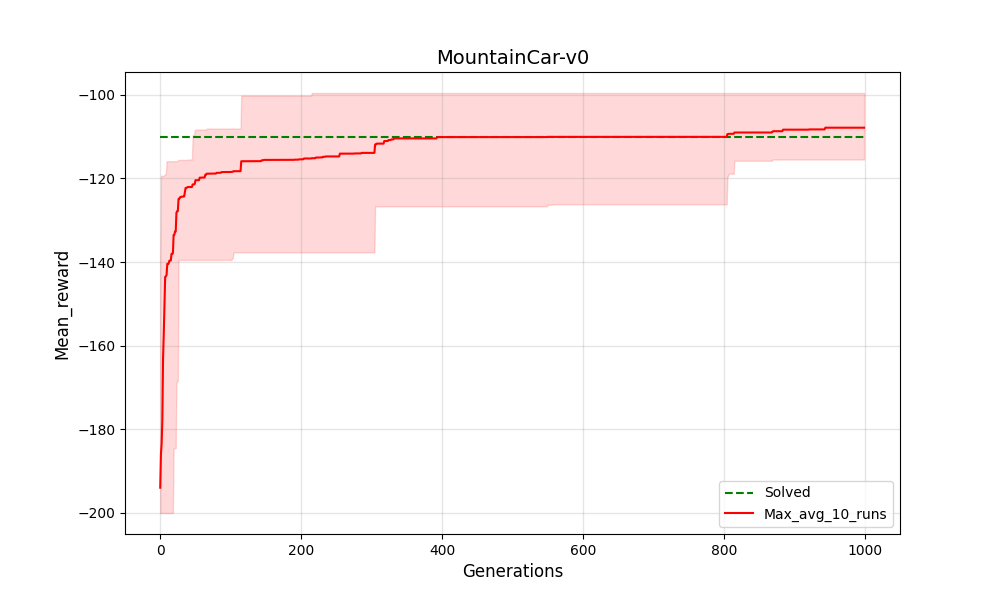
\includegraphics[width=1\linewidth]{images/MountainCar/MountainCar10run.png}
    \caption{Total training mean reward with orthogonal decision trees in the MountainCar-v0 environment, using both GE and PPO}
    \label{fig:MountainCarMean}
\end{figure}

\newpage

\begin{figure}[h!]
    \centering
    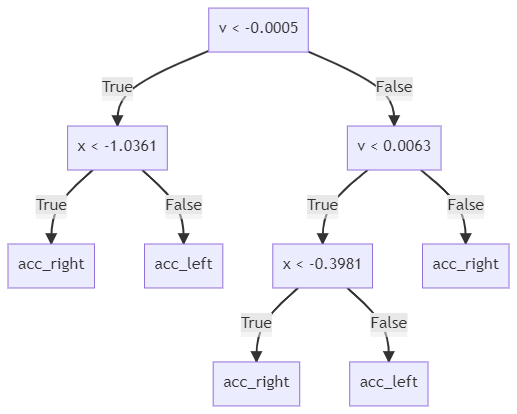
\includegraphics[width=0.5\linewidth]{images/MountainCar/bestPPOprunedMC.png}
    \caption{The best tree optimized by PPO in MountainCar-v0 environment, pruned by eliminating unnecessary branches}
    \label{fig:BestTreeMC}
\end{figure}

\newpage

\begin{figure}[h!]
    \centering
    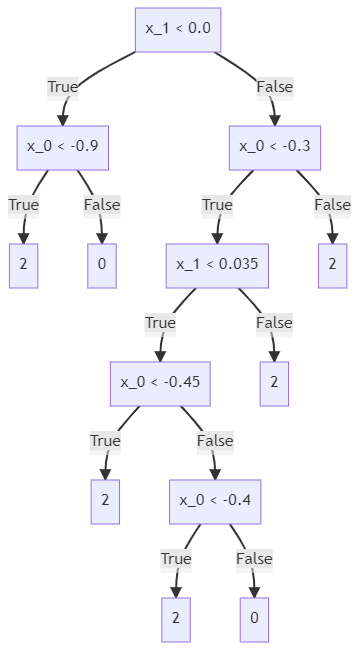
\includegraphics[width=0.4\linewidth]{images/MountainCar/bestLLCMC.png}
    \caption{The best tree obtained by L.L.Custode and G. Iacca in \cite{custode} in MountainCar-v0 environment}
    \label{fig:BestTreeLLCMC}
\end{figure}





\section{Interpretability study}
\label{sec:440}
All the obtained models are extremely easy to interpret, since they are all orthogonal DTs. Thus to determine the output given a particular state, it's necessary to check every time a Boolean condition and follow the branch accordingly until you reach a leaf where there's simply the action to take.

In the following sections, we evaluate the interpretability and the related measure of complexity, following the metric explained in Section \ref{sec:250}, of the best tree obtained via PPO for each environment.

\textit{Note:} having used oblique DTs (in which the split is composed of a linear combination of the input features and generates an oblique hyperplane) would have complicated a little the interpretability study, but would have also increased the performance of the models while still leading to more interpretable models than a neural network, as shown in \cite{custode}.

\subsection{CartPole-v1}
\label{subsec:441}
Looking at the model shown in Figure \ref{fig:BestTreeCP}, it's really easy to understand why the agent takes a decision in a particular state: 
\begin{itemize}
    \item the cart moves to the right when \[\theta < 0.0154 \land \omega > 0.2290\] or \[\theta > 0.0154\]
    \item the cart moves to the left o/w
\end{itemize}
The model, tested on 100 unseen episodes, obtained an $\mathcal{M}=35.60$, which is the same of the best tree obtained for CartPole-v1 in \cite{custode} (for the orthogonal DT).



\subsection{Acrobot-v1}
\label{subsec:442}
Looking now at the model in Figure \ref{fig:BestTreeAB} it's easy to say that:
\begin{itemize}
    \item torque +1 is applied when \[\omega_2 > 0.3094 \land \omega_1 > -2.9144\]
    \item torque -1 is applied when \[-14.2778 < \omega_2 < 0.3094 \land \omega_1 > -2.9144\] or \[\omega_2 < -14.2778\]
    \item torque 0 (do nothing) is applied o/w
\end{itemize}
The model, tested on 100 unseen episodes, obtained an $\mathcal{M}=53.4$, which is the same of the one obtained for the CartPole-v1 environment; in fact the tree has the same amount of decision nodes, but has a different structure (this type of tree is called \textit{Rule List}, like the one obtained in \cite{silva} for the LunarLander-v2 environment).


\subsection{MountainCar-v1}
\label{subsec:443}
Lastly, looking at the model in Figure \ref{fig:BestTreeMC}:
\begin{itemize}
    \item acceleration to the left is applied when \[ -0.0005 < \textit{v} < 0.0063 \land \textit{x} > -0.3981\] or \[\textit{v} < -0.0005 \land \textit{x} > -1.0361\]
    \item acceleration to the right is applied o/w
\end{itemize}
The model, tested on 100 unseen episodes, obtained an $\mathcal{M}=71.2$, which is higher w.r.t the ones obtained for the previous environments: this is because MountainCar is a more complex task compared with CartPole and Acrobot and need a more structured DT to be solved; in fact, in the configuration, it was specified that the maximum genotype length is 1024 (it was 100 for CartPole and Acrobot) and this leads to the possibility to obtain a more complex DT.

\newpage